\documentclass[a4paper,12pt]{article}
\usepackage{graphicx}
\usepackage{booktabs}
\usepackage{array}
\usepackage{listings}

\textheight=24.3cm
\topmargin=-1.8cm
\textwidth=16.7cm
\oddsidemargin=-0.3cm
\evensidemargin=0.0cm

\lstset{basicstyle=\ttfamily\footnotesize}

\title{CS-E4650 Methods of Data Mining, Exercise 2}
\author{Student Name (student id 000000)}
\date{}

\begin{document}
\maketitle

\section*{2.1 Comparison of PCA and spectral embedding}

\textbf{a)} Table~\ref{tab:summary} compares the two methods.

\begin{table}[!ht]
\centering
\caption{PCA dimension reduction and spectral embedding of $n\times d$ data
  $D$ into $k$ dimensions ($\lambda_1\le\dots\le\lambda_{\max}$).}
\label{tab:summary}
\begin{tabular}{>{\raggedright\arraybackslash}p{3.3cm}
  *{2}{>{\raggedright\arraybackslash}p{6cm}}}
\toprule
 & PCA dimension reduction & Spectral embedding \\
\midrule
optimization goal & maximize the variance of the data projected onto $k$
  orthogonal directions & minimize $\sum_{i,j}w_{ij}\|y_i-y_j\|^2
  =2\,\mathrm{tr}(Y^TLY)$ subject to $Y^TY=I$, i.e.\ keep similar points
  close \\
matrix for the eigendecomposition & covariance matrix
  $C=\frac{1}{n-1}D^TD$ of the mean-centred $D$ & Laplacian $L=\Lambda-W$
  of the similarity graph ($W$ weights, $\Lambda$ degrees) \\
size of the matrix & $d\times d$ & $n\times n$ \\
$k$ best eigenvalues & the $k$ largest, $\lambda_{\max-k+1},\dots,
  \lambda_{\max}$ & the $k$ smallest except $\lambda_1=0$, i.e.\
  $\lambda_2,\dots,\lambda_{k+1}$ \\
new data after transformation & $D'=DP_k$ ($n\times k$) with
  $P_k=[v_{\max-k+1},\dots,v_{\max}]$ & $Y=[v_2,\dots,v_{k+1}]$
  ($n\times k$), row $i$ represents point $i$ \\
\bottomrule
\end{tabular}
\end{table}

\textbf{b)} The largest distance between two points is
$d((0,0),(7,-2))=\sqrt{53}$. Dividing by it scales the similarities to
$[0,1]$, with 0 for the most distant pair. Numbering the points 1--6 in the
given order, their 2 nearest neighbours are $\{2,4\}$, $\{4,1\}$ (1 and 3
tie), $\{2,4\}$, $\{2,5\}$, $\{4,6\}$ and $\{5,4\}$. Joining two points when
either is among the 2 nearest neighbours of the other gives the edges 1--2,
2--3, 4--5 and 5--6 with similarity 0.717, 1--4 with 0.566, 2--4 with
0.752, 3--4 with 0.693 and 4--6 with 0.434. The tie does not matter,
because 2 is a nearest neighbour of both 1 and 3. The unnormalized
Laplacian $L=\Lambda-W$ and its eigendecomposition $L=V\,\mathrm{diag}
(\lambda)\,V^T$ are
\[
L=\left(\begin{array}{rrrrrr}
1.282 & -0.717 & 0 & -0.566 & 0 & 0\\
-0.717 & 2.186 & -0.717 & -0.752 & 0 & 0\\
0 & -0.717 & 1.410 & -0.693 & 0 & 0\\
-0.566 & -0.752 & -0.693 & 3.161 & -0.717 & -0.434\\
0 & 0 & 0 & -0.717 & 1.434 & -0.717\\
0 & 0 & 0 & -0.434 & -0.717 & 1.150
\end{array}\right),
\]
\[
V=\left(\begin{array}{rrrrrr}
0.408 & 0.390 & 0.711 & -0.044 & 0.399 & 0.120\\
0.408 & 0.344 & -0.027 & -0.039 & -0.796 & 0.282\\
0.408 & 0.334 & -0.700 & -0.076 & 0.443 & 0.173\\
0.408 & 0.036 & -0.041 & 0.105 & -0.098 & -0.900\\
0.408 & -0.493 & 0.013 & 0.727 & 0.047 & 0.244\\
0.408 & -0.611 & 0.043 & -0.672 & 0.005 & 0.080
\end{array}\right)
\]
with $\lambda=(0,\,0.598,\,1.342,\,1.993,\,2.851,\,3.839)$. The
1-dimensional embedding is the eigenvector of the second smallest
eigenvalue, $v_2=(0.390,\,0.344,\,0.334,\,0.036,\,-0.493,\,-0.611)$
(Figure~\ref{fig:embedding}b). The clusters are not mixed: points 1--3 lie
close together at 0.33--0.39 and points 4--6 below them, so one threshold
separates the clusters and the structure is preserved. Point 4 lies between
the clusters, nearer to points 1--3 than to 5 and 6, because it is the
nearest neighbour of point 2 and is linked to all points of the first
cluster.

\begin{figure}[!ht]
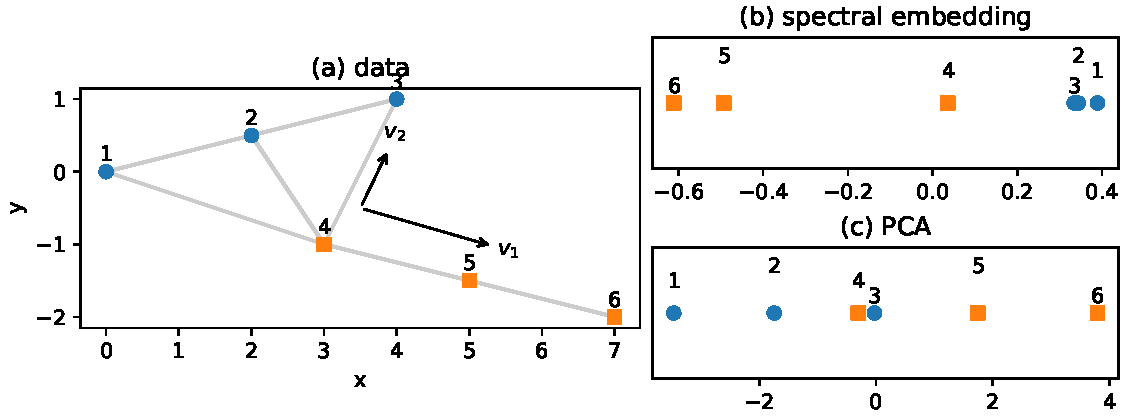
\includegraphics[width=\textwidth]{figures/embedding.pdf}
\caption{(a) Data (cluster 1 circles, cluster 2 squares), 2-nearest
  neighbour graph and PCA eigenvectors $v_1$, $v_2$ drawn from the mean.
  (b) 1-dimensional spectral embedding. (c) 1-dimensional PCA presentation.}
\label{fig:embedding}
\end{figure}

\textbf{c)} Along $v_1$, PCA orders the points 1, 2, 4, 3, 5, 6
(Figure~\ref{fig:embedding}c). Point 4 falls between points 2 and 3, so the
clusters overlap and the structure is lost, whereas spectral embedding
keeps them apart. PCA keeps the direction of largest variance. Both
clusters are elongated along the $x$-axis and overlap in $x$ (0--4 and
3--7), so $v_1$ runs along the clusters (Figure~\ref{fig:embedding}a). The
clusters are separated mainly in $y$ ($y\ge0$ versus $y<0$), a direction of
small variance that the 1-dimensional PCA discards. PCA is a global linear
projection that ignores which points are neighbours, whereas spectral
embedding preserves the similarity graph.

\section*{2.2 K-Means, K-Medians, and outliers}

\textbf{1.} Each iteration assigns every point to the nearest
representative and then updates the representatives (the mean for K-Means,
the median for K-Medians, with the mean of the two middle values for an
even number of points, although any value between them gives the same
clusters here). Table~\ref{tab:runs} lists all iterations.

\begin{table}[!ht]
\centering
\caption{Cluster labels of the points and representatives $c_1$, $c_2$
  after each iteration. The last iteration of each run changes nothing.}
\label{tab:runs}
\begin{tabular}{lcccccccccrr}
\toprule
Run & Iteration & 1 & 2 & 3 & 4 & 8 & 10 & 11 & 100 & $c_1$ & $c_2$ \\
\midrule
K-Means, (8), (11) & 1 & 1 & 1 & 1 & 1 & 1 & 2 & 2 & 2 & 3.6 & 40.33 \\
 & 2 & 1 & 1 & 1 & 1 & 1 & 1 & 1 & 2 & 5.57 & 100 \\
 & 3 & 1 & 1 & 1 & 1 & 1 & 1 & 1 & 2 & 5.57 & 100 \\
\midrule
K-Means, (1), (8) & 1 & 1 & 1 & 1 & 1 & 2 & 2 & 2 & 2 & 2.5 & 32.25 \\
 & 2 & 1 & 1 & 1 & 1 & 1 & 1 & 1 & 2 & 5.57 & 100 \\
 & 3 & 1 & 1 & 1 & 1 & 1 & 1 & 1 & 2 & 5.57 & 100 \\
\midrule
K-Medians, (8), (11) & 1 & 1 & 1 & 1 & 1 & 1 & 2 & 2 & 2 & 3 & 11 \\
 & 2 & 1 & 1 & 1 & 1 & 2 & 2 & 2 & 2 & 2.5 & 10.5 \\
 & 3 & 1 & 1 & 1 & 1 & 2 & 2 & 2 & 2 & 2.5 & 10.5 \\
\midrule
K-Medians, (1), (8) & 1 & 1 & 1 & 1 & 1 & 2 & 2 & 2 & 2 & 2.5 & 10.5 \\
 & 2 & 1 & 1 & 1 & 1 & 2 & 2 & 2 & 2 & 2.5 & 10.5 \\
\midrule
K-Medians, (1), (100) & 1 & 1 & 1 & 1 & 1 & 1 & 1 & 1 & 2 & 4 & 100 \\
 & 2 & 1 & 1 & 1 & 1 & 1 & 1 & 1 & 2 & 4 & 100 \\
\bottomrule
\end{tabular}
\end{table}

K-Means ends with $\{1,\dots,11\}$ and $\{100\}$ from both initializations.
The outlier pulls the mean of its cluster so far away that all other points
move to the other cluster, so the natural groups $\{1,2,3,4\}$ and
$\{8,10,11\}$ are merged. K-Medians is more robust. From (8), (11) and
(1), (8) it finds $\{1,2,3,4\}$ and $\{8,10,11,100\}$, because the outlier
hardly moves the median (10.5). With (1), (100), however, the outlier is a
representative from the start and forms a cluster of its own, which gives
the same clusters as K-Means. The initialization therefore matters, and with
$K=2$ an outlier can take a whole cluster.

\textbf{2.} With the $L_1$ distance $|x-y|$, Table~\ref{tab:silhouette}
gives $SC=0.192$ for \#1 and $SC=0.830$ for \#2.

\begin{table}[!ht]
\centering
\caption{Silhouettes with the $L_1$ distance, where $a$ averages over the
  other points of the cluster. The singleton $\{100\}$ in \#2 has $S=0$.}
\label{tab:silhouette}
\begin{tabular}{rrrrrrr}
\toprule
 & \multicolumn{3}{c}{Clustering \#1} & \multicolumn{3}{c}{Clustering \#2} \\
\cmidrule(lr){2-4}\cmidrule(lr){5-7}
$x$ & $a$ & $b$ & $S(x)$ & $a$ & $b$ & $S(x)$ \\
\midrule
1 & 2.00 & 31.25 & 0.936 & 5.33 & 99.00 & 0.946 \\
2 & 1.33 & 30.25 & 0.956 & 4.50 & 98.00 & 0.954 \\
3 & 1.33 & 29.25 & 0.954 & 4.00 & 97.00 & 0.959 \\
4 & 2.00 & 28.25 & 0.929 & 3.83 & 96.00 & 0.960 \\
8 & 32.33 & 5.50 & $-0.830$ & 4.50 & 92.00 & 0.951 \\
10 & 31.00 & 7.50 & $-0.758$ & 5.50 & 90.00 & 0.939 \\
11 & 31.00 & 8.50 & $-0.726$ & 6.33 & 89.00 & 0.929 \\
100 & 90.33 & 97.50 & 0.074 & & & 0 \\
\midrule
$SC$ & & & 0.192 & & & 0.830 \\
\bottomrule
\end{tabular}
\end{table}

SC thus strongly prefers \#2, which does not reflect the quality of the
clustering well. In \#2 the outlier is so far away that $b$ is very large
for all other points, so they get $S\approx0.95$ although the two natural
groups are merged, and the outlier itself gets $S=0$ as a singleton. In \#1
the outlier increases $a$ for 8, 10 and 11 and makes their silhouettes
negative although they form a natural group. Because the silhouette is
based on mean distances, it is dominated by the outlier and reflects its
separation rather than the structure of the other points.

\section*{2.3 Clustering validation with NMI}

$NMI=I(C,D)/\sqrt{H(C)H(D)}$ with $I(C,D)=\sum_{i,j}P(C_i,D_j)\log
\frac{P(C_i,D_j)}{P(C_i)P(D_j)}$ and $H(C)=-\sum_iP(C_i)\log P(C_i)$, where
the probabilities are relative frequencies. We use base-2 logarithms (NMI
does not depend on the base).

\textbf{a)} $P(C_1)=P(C_2)=P(\mathrm{mouse})=P(\mathrm{cat})=\frac12$ and
$P(C_1,\mathrm{mouse})=P(C_2,\mathrm{cat})=\frac12$, so
$I=2\cdot\frac12\log_2\frac{1/2}{1/4}=1$, $H(C)=H(D)=1$ and $NMI=1$.

\textbf{b)} Each pair $(C_i,D_j)$ contains one point, so
$P(C_i,D_j)=\frac14=P(C_i)P(D_j)$. Hence $I=0$ and $NMI=0$.

\textbf{c)} Now $P(C_i)=\frac14$ for the four clusters, so $H(C)=2$ and
$H(D)=1$. Each cluster lies in one class, so
$I=4\cdot\frac14\log_2\frac{1/4}{1/4\cdot1/2}=1$ and
$NMI=1/\sqrt2\approx0.71$. This is not intuitive. The classes are
irrelevant, yet NMI indicates a fairly strong agreement, because singleton
clusters are always pure and thus determine any classification completely.

\textbf{d)} Independence $P(C_i,D_j)=P(C_i)P(D_j)$ holds for the true
probabilities, but NMI uses relative frequencies in the data. With singleton
clusters these can never be independent: each cluster contains one point,
so $P(C_i,D_j)=1/n$ for the class of that point and 0 for the others,
whereas $P(C_i)P(D_j)=P(D_j)/n>0$. The estimated mutual information
therefore equals $H(D)>0$ although the classes carry no information. This
bias of the frequency estimates grows with the number of clusters, so NMI
favours many small clusters.

\section*{Appendix: Code}

\lstinputlisting{code/exercise2.py}

\end{document}
